\chapter*{Introduzione}
Da uno studio di ricerca avviato nei primi anni '90 sono stati esaminate le città e i loro progetti IT destinati agli spazi urbani. Da questo studio viene coniato anche il termine "Smart city".\cite{smart_city_terminology}\cite{smart:city_cybersecurity_privacy_cap2_1}

Parlare di Smart City significa pensare alla città del futuro in maniera integrata: ambiente, persone, tecnologie. In questo senso, la Smart City» si distingue dalla sorella più strettamente tecnologica, la città digitale, espressione che sottolinea il ruolo delle tecnologie informatiche. Tuttavia la città digitale è essenziale per la realizzazione della Smart City.

Nel mondo sempre più globale e interconnesso di oggi, sempre più persone decidono di vivere la propria vita nelle città. Nel 2018, il 55\% della popolazione mondiale risiede nelle aree urbane e entro il 2050, il 68 \% dovrebbe essere urbano. Nei prossimi decenni, sono previsti ulteriori aumenti sia della dimensione della popolazione urbana mondiale sia della sua quota sul totale. La diffusa crescita delle aree urbane descritta nella Revision of World Urbanization Prospects del 2018, lanciata dalla Divisione Popolazione dell'ONU DESA il 16 maggio 2018, evidenzia l'importanza di costruire città sostenibili, dove la crescita è pianificata e ben gestita.\cite{ONU_UDESA_urbanization}
In figura 1 viene mostrata la distribuzione di urbanizzazione nel mondo.
\begin{figure}[ht]
	\begin{center}
		\fbox{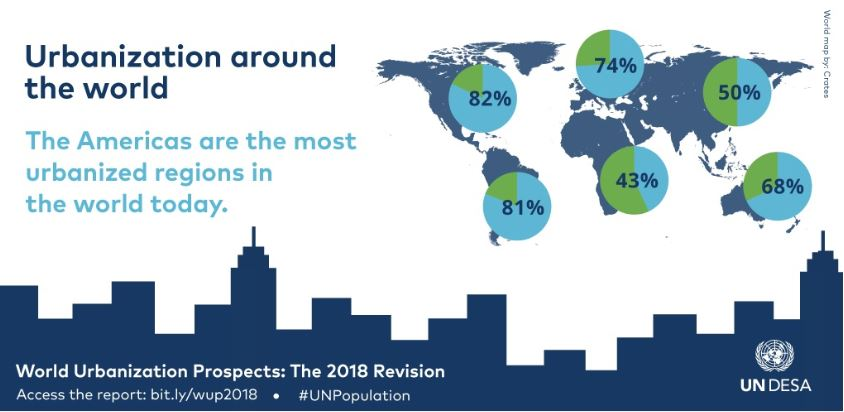
\includegraphics[width=320bp]{img/undesa.JPG}}
		\caption{Prospetto dell'urbanizzazione mondiale secodno Department of Economic and Social Affairs delle Nazioni Unite}
	\end{center}
\end{figure}

Da questi dati si evince che la rapida crescita della popolazione, sopratutto nelle città, comporta, da parte delle amministrazioni locali, una difficoltà nel gestire ed erogare servizi pubblici legati anche a problemi tecnologici orientati alle infrastrutture. Questi problemi diminuiscono la qualità del servizio rivolto al cittadino come ad esempio una elevata difficoltà nello smistamento dei rifiuti, problemi di viabilità con un aumento dell'inquinamento come consequenza. A questo va aggiunto ance la complessità nel gestire problemi sociali legati legati alla scarsa capacità di un comune di gestire le diverse classi sociali e di conseguenza ad un peggioramento della qualità della vita.\cite{What_make_city_smart}

Oltre alle problematiche infrastrutturali, le Smart City devono afrontare un problema di archiviazione e elaborazione delle informazioni. Per ottenere tale archiviazione, elaborazione e disponibilità dei dati, l'architettura necessita dell'aiuto di tecnologie sempre più evolute come il cloud computing\footnote{Il cloud computing è un paradigma di erogazione di servizi offerti on demand da un fornitore ad un cliente finale attraverso la rete Internet (come l'archiviazione, l'elaborazione o la trasmissione dati), a partire da un insieme di risorse preesistenti, configurabili e disponibili in remoto sotto forma di architettura distribuita.}.\cite{smart_problem_bigdata_1} \cite{smart_problem_bigdata_2}

\todo{gdm: potrebbe essere interessante? http://simonweckert.com/googlemapshacks.html}
